\documentclass[10pt]{article}
\usepackage[tmargin=1.25in,lmargin=1in,rmargin=1in,bmargin=1in,paper=letterpaper]{geometry}
\usepackage{amsmath,amssymb}
\usepackage{multirow,xcolor}
\usepackage{fancyhdr,ifthen,lastpage}
\usepackage{booktabs}
\usepackage{relsize}
\usepackage{enumitem}
\usepackage{empheq}
\usepackage{float}
\usepackage{amsthm}
\usepackage{changepage}
\usepackage{fancybox}
\usepackage{listings}
\usepackage{tikz}
\usepackage{tikz-qtree,tikz-qtree-compat}
\usepackage{hyperref}
\usepackage{mathtools}
% --------------------------------------------------------------------
% --------------------------------------------------------------------
\newcommand{\isdef}{\stackrel{\mathrm{def}}{=}}
\def\multiset#1#2{\ensuremath{\left(\kern-.3em\left(\genfrac{}{}{0pt}{}{#1}{#2}\right)\kern-.3em\right)}}
\newcommand\RR{{\mathbb R}}
\newcommand\CC{{\mathbb C}}
\newcommand\ZZ{{\mathbb Z}}
\newcommand\NN{{\mathbb N}}
\renewcommand\mod{{\textnormal{~mod~}}}
% --------------------------------------------------------------------
\newtheorem{theorem}{Theorem}[section]
\newtheorem{corollary}{Corollary}[theorem]
\newtheorem{lemma}[theorem]{Lemma}
\newtheorem*{remark}{Remark}
\theoremstyle{definition}
\newtheorem{definition}{Definition}[section]
\newtheorem{scholium}{Scholium}
\renewcommand\qedsymbol{$\blacksquare$}
\usepackage{cancel}

\usepackage{courier}

\definecolor{codegreen}{rgb}{0,0.6,0}
\definecolor{codegray}{rgb}{0.5,0.5,0.5}
\definecolor{codepurple}{rgb}{0.58,0,0.82}
\definecolor{backcolour}{rgb}{0.95,0.95,0.92}
 
\lstdefinestyle{mystyle}{
    backgroundcolor=\color{backcolour},   
    commentstyle=\color{codegreen},
    keywordstyle=\color{magenta},
    numberstyle=\tiny\color{codegray},
    stringstyle=\color{codepurple},
    basicstyle=\footnotesize\ttfamily,
    breakatwhitespace=false,         
    breaklines=true,                 
    captionpos=b,                    
    keepspaces=true,                 
    numbers=left,                    
    numbersep=5pt,                  
    showspaces=false,                
    showstringspaces=false,
    showtabs=false,                  
    tabsize=2
}
 
\lstset{style=mystyle}

\begin{document}
\pagestyle{fancy}

\setlength{\headheight}{0pt}
\setlength\parindent{0pt}

\lhead{ Math 55 - Spring \the\year}
\rhead{Forest Kobayashi}
\chead{\bf Math 55 Number Theory Notes}
\def\abs#1{\vert #1 \vert}
\def\set#1{\{ #1 \}}

\let\oldref\ref
\renewcommand{\ref}[1]{(\oldref{#1})}

\setlength{\headheight}{0pt}
\tableofcontents
% =====================================================================
\newpage
\section{Division, and Prime Numbers}
\subsection{Division} 
\begin{theorem}
For every $a\in \ZZ$ and $b \geq 1$, there exists some $q$ and $r$ such that 
\[ a = qb+r
\]
\end{theorem}
\begin{proof}
Consider $X = \set{a-bx:x\in\ZZ}_n\NN$, where "$_n\NN$" indicates that we are restricting the set to its nonnegative elements.  We want to claim: a) the set is nonempty, and b) the set has a lower bound.  \\~\\ 
For $a\geq 0$, then $x=0$ yields $a\in X$, and if $a$ is negative, then $x=a$ yields $(a-ba) = a(1-b)$.  $a$ is negative and $b\geq 1$, so $a(1-b)$ will be a negative number multiplied by something less than or equal to $0$, thus $a(1-b)$ is nonnegative.  \\~\\
So $X$ is always nonempty.  Let $r$ be the smallest element of $X$, and let $q$ be such that 
\[ a = qb+r
\]
Which implies $a - qb = r$.  Now, we show that $r$ is, at most, $(b-1)$ (i.e., $r\leq (b-1)$.  \\~\\
Suppose, to obtain a contradiction, that $r\geq b$.  Let $s=r-b$.  Then, $s\geq 0$, because $r\geq b$, and $s = a-(q+1)b \in X$.  So, we have now found a new smallest element of $X$ than $r$, which is a contradiction. 
\end{proof}
Associated with this operation is a relation. 
\subsection{Divisibility Relation}
\begin{definition}
$b|a$ (read "$b$ divides $a$" or "$b$ is a divisor of $a$" or "$a$ is a multiple of $b$") is defined by 
\[b|a \iff a = bx ~\textnormal{ for some $x\in \ZZ$}
\]
\end{definition}
This is equivalent (if $b$ is positive) to saying the remainder is zero independent of the signs of $a$ and $b$.  From this definition, we can say $0|0$.  If $0|a$, then $a$ \textit{must} be zero---there is no integer $x$ such that $0x=a\neq 0$.  A few things to note: 
\begin{enumerate}
\item The divides relation is reflexive: $a|a \forall a \in\ZZ$, with $q=1$.  
\item The divides relation is transitive: if $a|b$ and $b|c$, then $a|c$ $\forall a,b,c\in\ZZ$. Basically, we multiply by something, and then something else.  
\item If $d|a$, then $d|(a\cdot x) \forall x\in\ZZ$.  
\item If $d|a$ and $d|b$, then $d|(a+b)$
\item It follows 3. and 4. that if $d|a$ and $d|b$, then $d|(ax+by)\forall x,y\in\ZZ$.  This can be read as "$d$ divides any integer linear combination of $a$ and $b$."
\end{enumerate}
\subsection{Primes}
The number 1 can be thought of as the "basic building block of positive integers by addition."  I.e., if we have any positive integer $x$, we can construct $x$ by adding sufficiently many values of 1 together.  In a similar sense, primes are "the building blocks of positive integers by multiplication!"  
\begin{definition}{Prime:} a number $a\geq 2$ is said to be \textbf{prime} if the only positive integers that divide $a$ are 1 and $a$.  Note that we say here that we specify $a\geq 2$, so 1 is not a prime.  In a moment, we'll see that this is to make the Fundamental Theorem of Arithmetic cleaner.
\end{definition}
\begin{definition}{Composite:} a number $a\geq 2$ is \textbf{composite} if $a=bc$ for some $b\geq 2, ~c\geq 2$.  Basically, composite means that a number can be expressed as the product of two numbers, which can themselves be either prime or composite.  
\end{definition}
On the next page is a list of the primes between 0 and 900, with the primes in black.  Grey numbers are composite, and 0 and 1, being special cases, are written in blue.  If you can find a formula/pattern that will generate the $n^{th}$ prime, you will likely win the Fields medal and go down in history as having made the single largest contribution to mathematics that ever was.  But for now, we go on to prove a Lemma, to use in the proof of the fundamental theorem of arithmetic.
\begin{lemma}
For every integer $a \geq 2$, we have $p|a$ for some prime $p$.
\end{lemma}
\begin{proof}
(By contradiction): Suppose, to obtain a contradiction, that Lemma 1.2 is false, and let $a\geq 2$ be the smallest integer not divisible by any prime.  \\~\\
The number $a$ cannot itself be prime, because if it were, it would divide itself (because the division relation is reflexive), and would thus be divisible by a prime. \\~\\
Then $a$ must be composite.  Let $a=bc$ with $b\geq 2$ and $c\geq 2$.  Then $b$ is smaller than $a$, so $p|b$ for some prime $p$ (this is because we defined $a$ as the SMALLEST integer for which the Lemma fails, so any integer smaller than $a$ must satisfy the Lemma).  But then, since $b|a$, we have $p|a$, a contradiction.  So, there does not exist a smallest counterexample to the Lemma, so it must hold for all $a\geq 2$.    
\end{proof}
Now, we use Lemma 1.2 to prove a theorem.  
\begin{theorem}
There are (countably) infinitely many primes.  I.e., if $P$ is the set of primes, $|P| = \aleph_0$.
\end{theorem}
\begin{proof}(By contradiction):
We will only prove the infinite part, not the countably infinite part.  Suppose, to obtain a contradiction, that there are only finitely many primes, and list them 
\[(p_1,p_2,\dots,p_k)\]
Consider the number $N=p_1 p_2\cdots p_k+1$. $N$ is at least 2, because the smallest prime is $p_1=2$, so by the lemma, we have $q|N$ for some prime $q$.  The prime $q$ cannot be among the primes $p_1p_2\cdots p_k$, because since $N$ leaves a remainder of 0 when divided by $q$, but leaves a remainder of 1 when divided by any $p_i \in \set{p_1,p_2,\ldots,p_k}
$.  Thus, $q$ is a prime not among the $p_1\ldots p_k$, a contradiction.  \end{proof}
\subsection{Remarks}
\begin{itemize}
\item Divisibility is Reflexive and Transitive.  
\item However, it's not quite antisymmetric; for instance $-1|1$ and $1|-1$, but $-1\neq 1$.  
\item Something that's reflexive and transitive is called a \textbf{pre-order}. If we add in antisymmetric, we get an \textbf{order}.  
\item If $(a|b\land b|a)$, we define this as $a\equiv b$.  Note, this is an equivalence relation (i.e., it is reflexive, transitive, and symmetric).  
\item Equivalence classes partition a "universe of discourse" into sets of elements related by an equivalence relation.  Associates are members of the same equivalence classes.
\end{itemize}
\begin{figure}[h!]
\[
\begin{array}{cccccccccccccccccc}
\textcolor{blue}{0}&\textcolor{blue}{1}&2&3&\textcolor{gray}{4}&5&\textcolor{gray}{6}&7&\textcolor{gray}{8}&\textcolor{gray}{9}&\textcolor{gray}{10}&11&\textcolor{gray}{12}&13&\textcolor{gray}{14}&\textcolor{gray}{15}&\textcolor{gray}{16}&17\\\textcolor{gray}{18}&19&\textcolor{gray}{20}&\textcolor{gray}{21}&\textcolor{gray}{22}&23&\textcolor{gray}{24}&\textcolor{gray}{25}&\textcolor{gray}{26}&\textcolor{gray}{27}&\textcolor{gray}{28}&29&\textcolor{gray}{30}&31&\textcolor{gray}{32}&\textcolor{gray}{33}&\textcolor{gray}{34}&\textcolor{gray}{35}\\\textcolor{gray}{36}&37&\textcolor{gray}{38}&\textcolor{gray}{39}&\textcolor{gray}{40}&41&\textcolor{gray}{42}&43&\textcolor{gray}{44}&\textcolor{gray}{45}&\textcolor{gray}{46}&47&\textcolor{gray}{48}&\textcolor{gray}{49}&\textcolor{gray}{50}&\textcolor{gray}{51}&\textcolor{gray}{52}&53\\\textcolor{gray}{54}&\textcolor{gray}{55}&\textcolor{gray}{56}&\textcolor{gray}{57}&\textcolor{gray}{58}&59&\textcolor{gray}{60}&61&\textcolor{gray}{62}&\textcolor{gray}{63}&\textcolor{gray}{64}&\textcolor{gray}{65}&\textcolor{gray}{66}&67&\textcolor{gray}{68}&\textcolor{gray}{69}&\textcolor{gray}{70}&71\\\textcolor{gray}{72}&73&\textcolor{gray}{74}&\textcolor{gray}{75}&\textcolor{gray}{76}&\textcolor{gray}{77}&\textcolor{gray}{78}&79&\textcolor{gray}{80}&\textcolor{gray}{81}&\textcolor{gray}{82}&83&\textcolor{gray}{84}&\textcolor{gray}{85}&\textcolor{gray}{86}&\textcolor{gray}{87}&\textcolor{gray}{88}&89\\\textcolor{gray}{90}&\textcolor{gray}{91}&\textcolor{gray}{92}&\textcolor{gray}{93}&\textcolor{gray}{94}&\textcolor{gray}{95}&\textcolor{gray}{96}&97&\textcolor{gray}{98}&\textcolor{gray}{99}&\textcolor{gray}{100}&101&\textcolor{gray}{102}&103&\textcolor{gray}{104}&\textcolor{gray}{105}&\textcolor{gray}{106}&107\\\textcolor{gray}{108}&109&\textcolor{gray}{110}&\textcolor{gray}{111}&\textcolor{gray}{112}&113&\textcolor{gray}{114}&\textcolor{gray}{115}&\textcolor{gray}{116}&\textcolor{gray}{117}&\textcolor{gray}{118}&\textcolor{gray}{119}&\textcolor{gray}{120}&\textcolor{gray}{121}&\textcolor{gray}{122}&\textcolor{gray}{123}&\textcolor{gray}{124}&\textcolor{gray}{125}\\\textcolor{gray}{126}&127&\textcolor{gray}{128}&\textcolor{gray}{129}&\textcolor{gray}{130}&131&\textcolor{gray}{132}&\textcolor{gray}{133}&\textcolor{gray}{134}&\textcolor{gray}{135}&\textcolor{gray}{136}&137&\textcolor{gray}{138}&139&\textcolor{gray}{140}&\textcolor{gray}{141}&\textcolor{gray}{142}&\textcolor{gray}{143}\\\textcolor{gray}{144}&\textcolor{gray}{145}&\textcolor{gray}{146}&\textcolor{gray}{147}&\textcolor{gray}{148}&149&\textcolor{gray}{150}&151&\textcolor{gray}{152}&\textcolor{gray}{153}&\textcolor{gray}{154}&\textcolor{gray}{155}&\textcolor{gray}{156}&157&\textcolor{gray}{158}&\textcolor{gray}{159}&\textcolor{gray}{160}&\textcolor{gray}{161}\\\textcolor{gray}{162}&163&\textcolor{gray}{164}&\textcolor{gray}{165}&\textcolor{gray}{166}&167&\textcolor{gray}{168}&\textcolor{gray}{169}&\textcolor{gray}{170}&\textcolor{gray}{171}&\textcolor{gray}{172}&173&\textcolor{gray}{174}&\textcolor{gray}{175}&\textcolor{gray}{176}&\textcolor{gray}{177}&\textcolor{gray}{178}&179\\\textcolor{gray}{180}&181&\textcolor{gray}{182}&\textcolor{gray}{183}&\textcolor{gray}{184}&\textcolor{gray}{185}&\textcolor{gray}{186}&\textcolor{gray}{187}&\textcolor{gray}{188}&\textcolor{gray}{189}&\textcolor{gray}{190}&191&\textcolor{gray}{192}&193&\textcolor{gray}{194}&\textcolor{gray}{195}&\textcolor{gray}{196}&197\\\textcolor{gray}{198}&199&\textcolor{gray}{200}&\textcolor{gray}{201}&\textcolor{gray}{202}&\textcolor{gray}{203}&\textcolor{gray}{204}&\textcolor{gray}{205}&\textcolor{gray}{206}&\textcolor{gray}{207}&\textcolor{gray}{208}&\textcolor{gray}{209}&\textcolor{gray}{210}&211&\textcolor{gray}{212}&\textcolor{gray}{213}&\textcolor{gray}{214}&\textcolor{gray}{215}\\\textcolor{gray}{216}&\textcolor{gray}{217}&\textcolor{gray}{218}&\textcolor{gray}{219}&\textcolor{gray}{220}&\textcolor{gray}{221}&\textcolor{gray}{222}&223&\textcolor{gray}{224}&\textcolor{gray}{225}&\textcolor{gray}{226}&227&\textcolor{gray}{228}&229&\textcolor{gray}{230}&\textcolor{gray}{231}&\textcolor{gray}{232}&233\\\textcolor{gray}{234}&\textcolor{gray}{235}&\textcolor{gray}{236}&\textcolor{gray}{237}&\textcolor{gray}{238}&239&\textcolor{gray}{240}&241&\textcolor{gray}{242}&\textcolor{gray}{243}&\textcolor{gray}{244}&\textcolor{gray}{245}&\textcolor{gray}{246}&\textcolor{gray}{247}&\textcolor{gray}{248}&\textcolor{gray}{249}&\textcolor{gray}{250}&251\\\textcolor{gray}{252}&\textcolor{gray}{253}&\textcolor{gray}{254}&\textcolor{gray}{255}&\textcolor{gray}{256}&257&\textcolor{gray}{258}&\textcolor{gray}{259}&\textcolor{gray}{260}&\textcolor{gray}{261}&\textcolor{gray}{262}&263&\textcolor{gray}{264}&\textcolor{gray}{265}&\textcolor{gray}{266}&\textcolor{gray}{267}&\textcolor{gray}{268}&269\\\textcolor{gray}{270}&271&\textcolor{gray}{272}&\textcolor{gray}{273}&\textcolor{gray}{274}&\textcolor{gray}{275}&\textcolor{gray}{276}&277&\textcolor{gray}{278}&\textcolor{gray}{279}&\textcolor{gray}{280}&281&\textcolor{gray}{282}&283&\textcolor{gray}{284}&\textcolor{gray}{285}&\textcolor{gray}{286}&\textcolor{gray}{287}\\\textcolor{gray}{288}&\textcolor{gray}{289}&\textcolor{gray}{290}&\textcolor{gray}{291}&\textcolor{gray}{292}&293&\textcolor{gray}{294}&\textcolor{gray}{295}&\textcolor{gray}{296}&\textcolor{gray}{297}&\textcolor{gray}{298}&\textcolor{gray}{299}&\textcolor{gray}{300}&\textcolor{gray}{301}&\textcolor{gray}{302}&\textcolor{gray}{303}&\textcolor{gray}{304}&\textcolor{gray}{305}\\\textcolor{gray}{306}&307&\textcolor{gray}{308}&\textcolor{gray}{309}&\textcolor{gray}{310}&311&\textcolor{gray}{312}&313&\textcolor{gray}{314}&\textcolor{gray}{315}&\textcolor{gray}{316}&317&\textcolor{gray}{318}&\textcolor{gray}{319}&\textcolor{gray}{320}&\textcolor{gray}{321}&\textcolor{gray}{322}&\textcolor{gray}{323}\\\textcolor{gray}{324}&\textcolor{gray}{325}&\textcolor{gray}{326}&\textcolor{gray}{327}&\textcolor{gray}{328}&\textcolor{gray}{329}&\textcolor{gray}{330}&331&\textcolor{gray}{332}&\textcolor{gray}{333}&\textcolor{gray}{334}&\textcolor{gray}{335}&\textcolor{gray}{336}&337&\textcolor{gray}{338}&\textcolor{gray}{339}&\textcolor{gray}{340}&\textcolor{gray}{341}\\\textcolor{gray}{342}&\textcolor{gray}{343}&\textcolor{gray}{344}&\textcolor{gray}{345}&\textcolor{gray}{346}&347&\textcolor{gray}{348}&349&\textcolor{gray}{350}&\textcolor{gray}{351}&\textcolor{gray}{352}&353&\textcolor{gray}{354}&\textcolor{gray}{355}&\textcolor{gray}{356}&\textcolor{gray}{357}&\textcolor{gray}{358}&359\\\textcolor{gray}{360}&\textcolor{gray}{361}&\textcolor{gray}{362}&\textcolor{gray}{363}&\textcolor{gray}{364}&\textcolor{gray}{365}&\textcolor{gray}{366}&367&\textcolor{gray}{368}&\textcolor{gray}{369}&\textcolor{gray}{370}&\textcolor{gray}{371}&\textcolor{gray}{372}&373&\textcolor{gray}{374}&\textcolor{gray}{375}&\textcolor{gray}{376}&\textcolor{gray}{377}\\\textcolor{gray}{378}&379&\textcolor{gray}{380}&\textcolor{gray}{381}&\textcolor{gray}{382}&383&\textcolor{gray}{384}&\textcolor{gray}{385}&\textcolor{gray}{386}&\textcolor{gray}{387}&\textcolor{gray}{388}&389&\textcolor{gray}{390}&\textcolor{gray}{391}&\textcolor{gray}{392}&\textcolor{gray}{393}&\textcolor{gray}{394}&\textcolor{gray}{395}\\\textcolor{gray}{396}&397&\textcolor{gray}{398}&\textcolor{gray}{399}&\textcolor{gray}{400}&401&\textcolor{gray}{402}&\textcolor{gray}{403}&\textcolor{gray}{404}&\textcolor{gray}{405}&\textcolor{gray}{406}&\textcolor{gray}{407}&\textcolor{gray}{408}&409&\textcolor{gray}{410}&\textcolor{gray}{411}&\textcolor{gray}{412}&\textcolor{gray}{413}\\\textcolor{gray}{414}&\textcolor{gray}{415}&\textcolor{gray}{416}&\textcolor{gray}{417}&\textcolor{gray}{418}&419&\textcolor{gray}{420}&421&\textcolor{gray}{422}&\textcolor{gray}{423}&\textcolor{gray}{424}&\textcolor{gray}{425}&\textcolor{gray}{426}&\textcolor{gray}{427}&\textcolor{gray}{428}&\textcolor{gray}{429}&\textcolor{gray}{430}&431\\\textcolor{gray}{432}&433&\textcolor{gray}{434}&\textcolor{gray}{435}&\textcolor{gray}{436}&\textcolor{gray}{437}&\textcolor{gray}{438}&439&\textcolor{gray}{440}&\textcolor{gray}{441}&\textcolor{gray}{442}&443&\textcolor{gray}{444}&\textcolor{gray}{445}&\textcolor{gray}{446}&\textcolor{gray}{447}&\textcolor{gray}{448}&449\\\textcolor{gray}{450}&\textcolor{gray}{451}&\textcolor{gray}{452}&\textcolor{gray}{453}&\textcolor{gray}{454}&\textcolor{gray}{455}&\textcolor{gray}{456}&457&\textcolor{gray}{458}&\textcolor{gray}{459}&\textcolor{gray}{460}&461&\textcolor{gray}{462}&463&\textcolor{gray}{464}&\textcolor{gray}{465}&\textcolor{gray}{466}&467\\\textcolor{gray}{468}&\textcolor{gray}{469}&\textcolor{gray}{470}&\textcolor{gray}{471}&\textcolor{gray}{472}&\textcolor{gray}{473}&\textcolor{gray}{474}&\textcolor{gray}{475}&\textcolor{gray}{476}&\textcolor{gray}{477}&\textcolor{gray}{478}&479&\textcolor{gray}{480}&\textcolor{gray}{481}&\textcolor{gray}{482}&\textcolor{gray}{483}&\textcolor{gray}{484}&\textcolor{gray}{485}\\\textcolor{gray}{486}&487&\textcolor{gray}{488}&\textcolor{gray}{489}&\textcolor{gray}{490}&491&\textcolor{gray}{492}&\textcolor{gray}{493}&\textcolor{gray}{494}&\textcolor{gray}{495}&\textcolor{gray}{496}&\textcolor{gray}{497}&\textcolor{gray}{498}&499&\textcolor{gray}{500}&\textcolor{gray}{501}&\textcolor{gray}{502}&503\\\textcolor{gray}{504}&\textcolor{gray}{505}&\textcolor{gray}{506}&\textcolor{gray}{507}&\textcolor{gray}{508}&509&\textcolor{gray}{510}&\textcolor{gray}{511}&\textcolor{gray}{512}&\textcolor{gray}{513}&\textcolor{gray}{514}&\textcolor{gray}{515}&\textcolor{gray}{516}&\textcolor{gray}{517}&\textcolor{gray}{518}&\textcolor{gray}{519}&\textcolor{gray}{520}&521\\\textcolor{gray}{522}&523&\textcolor{gray}{524}&\textcolor{gray}{525}&\textcolor{gray}{526}&\textcolor{gray}{527}&\textcolor{gray}{528}&\textcolor{gray}{529}&\textcolor{gray}{530}&\textcolor{gray}{531}&\textcolor{gray}{532}&\textcolor{gray}{533}&\textcolor{gray}{534}&\textcolor{gray}{535}&\textcolor{gray}{536}&\textcolor{gray}{537}&\textcolor{gray}{538}&\textcolor{gray}{539}\\\textcolor{gray}{540}&541&\textcolor{gray}{542}&\textcolor{gray}{543}&\textcolor{gray}{544}&\textcolor{gray}{545}&\textcolor{gray}{546}&547&\textcolor{gray}{548}&\textcolor{gray}{549}&\textcolor{gray}{550}&\textcolor{gray}{551}&\textcolor{gray}{552}&\textcolor{gray}{553}&\textcolor{gray}{554}&\textcolor{gray}{555}&\textcolor{gray}{556}&557\\\textcolor{gray}{558}&\textcolor{gray}{559}&\textcolor{gray}{560}&\textcolor{gray}{561}&\textcolor{gray}{562}&563&\textcolor{gray}{564}&\textcolor{gray}{565}&\textcolor{gray}{566}&\textcolor{gray}{567}&\textcolor{gray}{568}&569&\textcolor{gray}{570}&571&\textcolor{gray}{572}&\textcolor{gray}{573}&\textcolor{gray}{574}&\textcolor{gray}{575}\\\textcolor{gray}{576}&577&\textcolor{gray}{578}&\textcolor{gray}{579}&\textcolor{gray}{580}&\textcolor{gray}{581}&\textcolor{gray}{582}&\textcolor{gray}{583}&\textcolor{gray}{584}&\textcolor{gray}{585}&\textcolor{gray}{586}&587&\textcolor{gray}{588}&\textcolor{gray}{589}&\textcolor{gray}{590}&\textcolor{gray}{591}&\textcolor{gray}{592}&593\\\textcolor{gray}{594}&\textcolor{gray}{595}&\textcolor{gray}{596}&\textcolor{gray}{597}&\textcolor{gray}{598}&599&\textcolor{gray}{600}&601&\textcolor{gray}{602}&\textcolor{gray}{603}&\textcolor{gray}{604}&\textcolor{gray}{605}&\textcolor{gray}{606}&607&\textcolor{gray}{608}&\textcolor{gray}{609}&\textcolor{gray}{610}&\textcolor{gray}{611}\\\textcolor{gray}{612}&613&\textcolor{gray}{614}&\textcolor{gray}{615}&\textcolor{gray}{616}&617&\textcolor{gray}{618}&619&\textcolor{gray}{620}&\textcolor{gray}{621}&\textcolor{gray}{622}&\textcolor{gray}{623}&\textcolor{gray}{624}&\textcolor{gray}{625}&\textcolor{gray}{626}&\textcolor{gray}{627}&\textcolor{gray}{628}&\textcolor{gray}{629}\\\textcolor{gray}{630}&631&\textcolor{gray}{632}&\textcolor{gray}{633}&\textcolor{gray}{634}&\textcolor{gray}{635}&\textcolor{gray}{636}&\textcolor{gray}{637}&\textcolor{gray}{638}&\textcolor{gray}{639}&\textcolor{gray}{640}&641&\textcolor{gray}{642}&643&\textcolor{gray}{644}&\textcolor{gray}{645}&\textcolor{gray}{646}&647\\\textcolor{gray}{648}&\textcolor{gray}{649}&\textcolor{gray}{650}&\textcolor{gray}{651}&\textcolor{gray}{652}&653&\textcolor{gray}{654}&\textcolor{gray}{655}&\textcolor{gray}{656}&\textcolor{gray}{657}&\textcolor{gray}{658}&659&\textcolor{gray}{660}&661&\textcolor{gray}{662}&\textcolor{gray}{663}&\textcolor{gray}{664}&\textcolor{gray}{665}\\\textcolor{gray}{666}&\textcolor{gray}{667}&\textcolor{gray}{668}&\textcolor{gray}{669}&\textcolor{gray}{670}&\textcolor{gray}{671}&\textcolor{gray}{672}&673&\textcolor{gray}{674}&\textcolor{gray}{675}&\textcolor{gray}{676}&677&\textcolor{gray}{678}&\textcolor{gray}{679}&\textcolor{gray}{680}&\textcolor{gray}{681}&\textcolor{gray}{682}&683\\\textcolor{gray}{684}&\textcolor{gray}{685}&\textcolor{gray}{686}&\textcolor{gray}{687}&\textcolor{gray}{688}&\textcolor{gray}{689}&\textcolor{gray}{690}&691&\textcolor{gray}{692}&\textcolor{gray}{693}&\textcolor{gray}{694}&\textcolor{gray}{695}&\textcolor{gray}{696}&\textcolor{gray}{697}&\textcolor{gray}{698}&\textcolor{gray}{699}&\textcolor{gray}{700}&701\\\textcolor{gray}{702}&\textcolor{gray}{703}&\textcolor{gray}{704}&\textcolor{gray}{705}&\textcolor{gray}{706}&\textcolor{gray}{707}&\textcolor{gray}{708}&709&\textcolor{gray}{710}&\textcolor{gray}{711}&\textcolor{gray}{712}&\textcolor{gray}{713}&\textcolor{gray}{714}&\textcolor{gray}{715}&\textcolor{gray}{716}&\textcolor{gray}{717}&\textcolor{gray}{718}&719\\\textcolor{gray}{720}&\textcolor{gray}{721}&\textcolor{gray}{722}&\textcolor{gray}{723}&\textcolor{gray}{724}&\textcolor{gray}{725}&\textcolor{gray}{726}&727&\textcolor{gray}{728}&\textcolor{gray}{729}&\textcolor{gray}{730}&\textcolor{gray}{731}&\textcolor{gray}{732}&733&\textcolor{gray}{734}&\textcolor{gray}{735}&\textcolor{gray}{736}&\textcolor{gray}{737}\\\textcolor{gray}{738}&739&\textcolor{gray}{740}&\textcolor{gray}{741}&\textcolor{gray}{742}&743&\textcolor{gray}{744}&\textcolor{gray}{745}&\textcolor{gray}{746}&\textcolor{gray}{747}&\textcolor{gray}{748}&\textcolor{gray}{749}&\textcolor{gray}{750}&751&\textcolor{gray}{752}&\textcolor{gray}{753}&\textcolor{gray}{754}&\textcolor{gray}{755}\\\textcolor{gray}{756}&757&\textcolor{gray}{758}&\textcolor{gray}{759}&\textcolor{gray}{760}&761&\textcolor{gray}{762}&\textcolor{gray}{763}&\textcolor{gray}{764}&\textcolor{gray}{765}&\textcolor{gray}{766}&\textcolor{gray}{767}&\textcolor{gray}{768}&769&\textcolor{gray}{770}&\textcolor{gray}{771}&\textcolor{gray}{772}&773\\\textcolor{gray}{774}&\textcolor{gray}{775}&\textcolor{gray}{776}&\textcolor{gray}{777}&\textcolor{gray}{778}&\textcolor{gray}{779}&\textcolor{gray}{780}&\textcolor{gray}{781}&\textcolor{gray}{782}&\textcolor{gray}{783}&\textcolor{gray}{784}&\textcolor{gray}{785}&\textcolor{gray}{786}&787&\textcolor{gray}{788}&\textcolor{gray}{789}&\textcolor{gray}{790}&\textcolor{gray}{791}\\\textcolor{gray}{792}&\textcolor{gray}{793}&\textcolor{gray}{794}&\textcolor{gray}{795}&\textcolor{gray}{796}&797&\textcolor{gray}{798}&\textcolor{gray}{799}&\textcolor{gray}{800}&\textcolor{gray}{801}&\textcolor{gray}{802}&\textcolor{gray}{803}&\textcolor{gray}{804}&\textcolor{gray}{805}&\textcolor{gray}{806}&\textcolor{gray}{807}&\textcolor{gray}{808}&809\\\textcolor{gray}{810}&811&\textcolor{gray}{812}&\textcolor{gray}{813}&\textcolor{gray}{814}&\textcolor{gray}{815}&\textcolor{gray}{816}&\textcolor{gray}{817}&\textcolor{gray}{818}&\textcolor{gray}{819}&\textcolor{gray}{820}&821&\textcolor{gray}{822}&823&\textcolor{gray}{824}&\textcolor{gray}{825}&\textcolor{gray}{826}&827\\\textcolor{gray}{828}&829&\textcolor{gray}{830}&\textcolor{gray}{831}&\textcolor{gray}{832}&\textcolor{gray}{833}&\textcolor{gray}{834}&\textcolor{gray}{835}&\textcolor{gray}{836}&\textcolor{gray}{837}&\textcolor{gray}{838}&839&\textcolor{gray}{840}&\textcolor{gray}{841}&\textcolor{gray}{842}&\textcolor{gray}{843}&\textcolor{gray}{844}&\textcolor{gray}{845}\\\textcolor{gray}{846}&\textcolor{gray}{847}&\textcolor{gray}{848}&\textcolor{gray}{849}&\textcolor{gray}{850}&\textcolor{gray}{851}&\textcolor{gray}{852}&853&\textcolor{gray}{854}&\textcolor{gray}{855}&\textcolor{gray}{856}&857&\textcolor{gray}{858}&859&\textcolor{gray}{860}&\textcolor{gray}{861}&\textcolor{gray}{862}&863\\\textcolor{gray}{864}&\textcolor{gray}{865}&\textcolor{gray}{866}&\textcolor{gray}{867}&\textcolor{gray}{868}&\textcolor{gray}{869}&\textcolor{gray}{870}&\textcolor{gray}{871}&\textcolor{gray}{872}&\textcolor{gray}{873}&\textcolor{gray}{874}&\textcolor{gray}{875}&\textcolor{gray}{876}&877&\textcolor{gray}{878}&\textcolor{gray}{879}&\textcolor{gray}{880}&881\\\textcolor{gray}{882}&883&\textcolor{gray}{884}&\textcolor{gray}{885}&\textcolor{gray}{886}&887&\textcolor{gray}{888}&\textcolor{gray}{889}&\textcolor{gray}{890}&\textcolor{gray}{891}&\textcolor{gray}{892}&\textcolor{gray}{893}&\textcolor{gray}{894}&\textcolor{gray}{895}&\textcolor{gray}{896}&\textcolor{gray}{897}&\textcolor{gray}{898}&\textcolor{gray}{899}
\end{array}
\]
\end{figure}
\clearpage
\section{The Fundamental Theorem of Arithmetic, GCD, and LCM}
\subsection{The Fundamental Theorem of Arithmetic and Corollaries}
\begin{theorem}[The Fundamental Theorem of Arithmetic]
Every integer $a\geq 1$ is the product of the primes in a unique multiset of primes.
\end{theorem}
\begin{proof}[Existence proof](By Strong Induction) We first prove the existence part---that is, that $a$ has a prime factorization
\[ 
a = p_1 p_2\ldots p_i \textnormal{~for primes $p_1,p_2,\ldots,p_i$}
\]
We proceed by strong Induction.  For the base case, $a=1$, we can take $i=0$, i.e. the number corresponding to the empty multiset $\langle \rangle$.  The product of the empty multiset is 1, so $1$ can be expressed as a multiset of primes, namely the empty multiset.  For the inductive step, we now consider $a\geq 2$ (as we have disposed of 1).  We assume the existence of a prime factorization for all positive integers strictly less than $a$, and prove for $a$.  If $a\geq 2$ is prime, then we can take $i=1$, and $p_1=a$.  I.e., we can express $a$ as the product of a multiset just containing itself.  Otherwise, if $a$ is composite, then we can express $a$ as the product of two numbers $bc$ with $b\geq 2,~c\geq 2$.  Because neither $b$ nor $c$ is 1, then we must have that $a>b$ and $a>c$, because $b$ and $c$ at the very least divide $a$ in two.  Thus, by the inductive hypothesis, $b$ and $c$ have prime factorizations 
\begin{align*}
b &= q_1 q_2\ldots q_j & c &= r_1 r_2\ldots r_k
\end{align*}
And thus 
\[a = q_1q_2\ldots q_j r_1 r_2 \ldots r_k = b\cdot c
\]
Thus, by the Principle of Mathematical Induction (strong version), every integer $a\geq 1$ can be written as the product of the primes in a multiset of primes.
\end{proof}~\\
\begin{proof}[Uniqueness proof](By Contradiction) Now, we prove uniqueness.  Suppose, to obtain a contradiction, that uniqueness fails, and by the well ordering principle, we can focus on a number $n$, the smallest possitive integer that has two distinct factorizations. 
\begin{align*}
n &= p_1 p_2 \ldots p_i & n&= q_1 q_2 \ldots q_j 
\end{align*}
None of the $p$'s can be the same as any of the $q$'s, otherwise we could divide both factorizations of $n$ by the common prime, and obtain a smaller counterexample.  \\~\\
Without loss of generality, $p_1$ is the smallest of $p$'s $p_1\ldots p_i$, and $q_1$ is the smallest of the $q$'s $q_1\ldots q_j$, and $p_1<q_1$.  (N.B.---this is a perfectly fine thing to stipulate, and \textbf{does not affect the validity of the proof or restrict our values of $n$ in any way.}  It is equivalent to stating "call the smallest of the $p$'s $p_1$ and the second smallest $p_2$ $\ldots$ and do the same with the $q$'s, then switch which ones are labled as $p$ or $q$ depending on which has the smaller smallest element.)  \\~\\
Now, consider $m=p_1(q_2\ldots q_j$).  Then, we have $1\leq m < n$, because $p_1$ is strictly less than $q_1$. Thus, $n-m$, which is 
\[n-m = (q_1-p_1)q_2\ldots q_j\]
Is strictly smaller than $n$, so it must have a unique factorization into primes.  We will obtain a contradiction by finding two different factorizations for $n-m$.\\~\\
Since $p_1|m$ and $p_1|n$, it divides their integer linear combination (i.e., $p|(n-m)$), so we have 
\begin{equation}\label{eq:factorization 1}
(n-m) = p_1(r_1\ldots r_k)
\end{equation}
When $r_1\ldots r_k$ is a factorization of $\frac{n-m}{p_1}$.  On the other hand, we have 
\begin{equation}\label{eq:factorization 2}
(n-m) = s_1\ldots s_\ell q_1\ldots q_j
\end{equation}
where $s_1\ldots s_\ell$ is a factorization of $q_1-p_1$.  We now now want to find a prime that occurs in \ref{eq:factorization 1} but not \ref{eq:factorization 2}.  $p_1$ can't be any of the $q$'s, as noted before.  But also, it's not among the $s$'s, because $p_1 \nmid (q_1-p_1)$ because $p_1\nmid q_1$ (no prime divides another prime).  \\~\\
Thus, \ref{eq:factorization 1} and \ref{eq:factorization 2} are different factorizations of $n-m$, so we've found a new smallest number that cannot be written as a unique product of primes, a contradiction.  Thus, every number $a\geq 1$ can be written as the product of the primes in a \textit{unique} multiset of primes.
\end{proof}
\begin{corollary}
Suppose $a$ and $b$ are positive integers, and $p$ is prime.  If $p|ab$, then either $p|a$, or $p|b$, or both.  It's essential that $p$ is a prime---for instance, $4|(2\cdot 6)$, but $4\nmid 2$, $4\nmid 6$.  
\end{corollary}
\begin{proof}
Let $a=q_1\ldots q_i$ and $b=r_1\ldots r_j$ be the factorization of $a$ and $b$ into primes.  Then, 
\begin{equation}\label{eq:ab factorization}
ab = q_1\ldots q_i r_1\ldots r_j
\end{equation}
is the "unique" factorization of $ab$.  Since $p|ab$, then 
\begin{equation} \label{eq:ab factorization 2}
ab=p(s_1\ldots s_k) 
\end{equation}
where $s_1\ldots s_k$ is the factorization of $\frac{ab}{p}$.  Then, $p$ appears in \ref{eq:ab factorization} or \ref{eq:ab factorization 2}, and thus $p$ divides $a$ or $b$. (N.B.---that's an inclusive or!)
\end{proof}
\subsection{GCD and LCM}
Let's consider the orders of addition and division over the positiver integers.  
\begin{figure}[H]
\begin{minipage}{.5\textwidth}
\centering
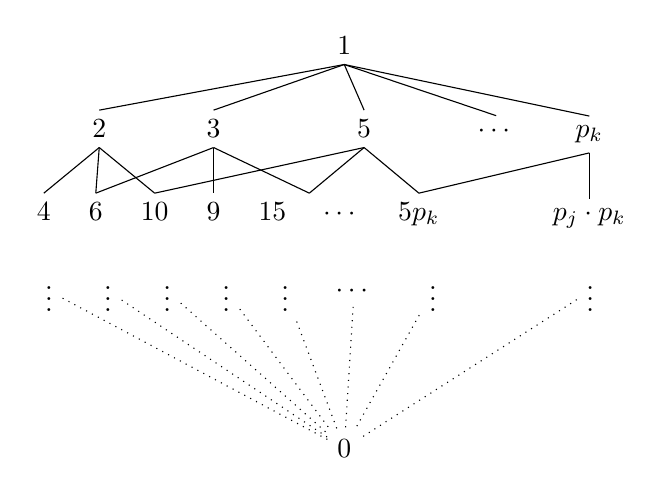
\begin{tikzpicture}[sibling distance=.25cm]
\Tree [.\node (1) {1};
      	[.\node (2) {2}; [.4 ] [.\node (6) {6}; ][.\node (10) {10}; ]]
        [.\node (3) {3}; [.9 ] ]
        [.\node (5) {5}; [.\node (15) {15$~~~~\cdots$}; ] [.\node (5pk) {$5p_k$}; ]]
        [.\node (dots) {$\cdots$}; ] 
        [.\node (pk) {$p_k$}; [.\node (pjpk) {$p_j\cdot p_k$}; ] ] ]
\draw (3.south) -- (6.north);
\draw (3.south) -- (15.north);
\draw (5.south) -- (10.north);
\draw (pk.south) -- (5pk.north);
\node (o) at (0,-5) {0};
\foreach \x in {-3.75,-3,...,-.75}{
	\node (vdots) at (\x, -3) {$\vdots$};
	\draw[dotted] (vdots) -- (o);}
\node (hdots) at (.125, -3) {$\cdots$};
\draw[dotted] (hdots) -- (o);
\node (morevdots) at (1.125,-3) {$\vdots$};
\draw[dotted] (morevdots) -- (o);
\node (evenmorevdots) at (3.125,-3) {$\vdots$};
\draw[dotted] (evenmorevdots) -- (o); 
\end{tikzpicture}
\caption{The order of division.  Note that numbers in the $n^{th}$ row have $n$ prime factors.  Any positive integer divides $0$, so $0$ is at the "top" (yes it's mirrored here I know) of the order.}
\end{minipage}
\begin{minipage}{.5\textwidth}
\centering
\begin{tikzpicture}
\Tree[.0
        [.1
        [.\node (2) {2}; 
           [.3 [.\node (vdots){$\vdots$};[.\node (inf){$\infty$};]]
           ]]]] 
\end{tikzpicture}
\caption{The order of addition}
\end{minipage}
\end{figure}
Notice that when considering the construction of integers by multiplication, we have to think a lot less linearly.  Thus, in the following cases, we'll have to be sure we treat 0 as a special case, so we'll deal initially with values of $a$ that are greater than or equal to 1.    \\~\\~\\
Suppose $a\geq 1$.  Then 
\begin{equation}\label{eq:alpha factorization for a}
a = 2^{\alpha_2}\cdot 3^{\alpha_3} \cdot 5^{\alpha_5} \cdots p^{\alpha_p} \cdots 
\end{equation}
Where the $\alpha$'s are natural numbers greater than or equal to 0, where each $\alpha$ tells us how many times each prime appears in the prime factorization. Note that for $a\in\NN$, for any prime $p$, $\alpha_p\geq 0$, but $\alpha_p\geq 1$ for only finitely many $p$.  Let us define $b$ similarly: 
\begin{equation}
b = 2^{\beta_2}\cdot 3^{\beta_3} \cdot 5^{\beta_5} \cdots p^{\beta_p}\cdots 
\end{equation}
Then, 
\begin{equation}\label{eq: alpha plus beta factorization of ab}
ab = 2^{\alpha_2 + \beta_2} \cdot 3^{\alpha_3 + \beta_3} \cdot 5^{\alpha_5 + \beta_5} \cdots p^{\alpha_p + \beta_p} \cdots 
\end{equation}
Furthermore, $b|a$ iff $\beta_p \leq \alpha_p~~ \forall p$ where $p$ is a prime, and in this case, if $b|a$, then $\frac{a}{b}$ is an integer, and we can find it in a similar manner to \ref{eq: alpha plus beta factorization of ab} by taking 
\begin{equation}
\frac{a}{b}= 2^{\alpha_2 - \beta_2} \cdot 3^{\alpha_3 - \beta_3} \cdot 5^{\alpha_5 - \beta_5} \cdots p^{\alpha_p - \beta_p} \cdots 
\end{equation}
Given $a$ and $b$, we can introduce the \textbf{least common multiple} of $a$ and $b$ (denoted $[a,b]$), the smallest positive integer for which $a$ and $b$ are both divisors
\begin{definition}[Least Common Multiple]
\begin{equation} \label{lcm def}
[a,b] = 2^{\textnormal{max}(\alpha_2,\beta_2)}\cdot 3^{\textnormal{max}(\alpha_3,\beta_3)}\cdot 5^{\textnormal{max}(\alpha_5,\beta_5)}\cdots p^{\textnormal{max}(\alpha_p,\beta_p)}\cdots 
\end{equation}
\end{definition}
\noindent So $a|[a,b]$ and $b|[a,b]$.  Note that if $a|c$ and $b|c$, then it must be true that $[a,b]|c$.  \\~\\Similarly, we introduce the \textbf{greatest common divisor} of $a$ and $b$ (denoted $(a,b)$), the largest positive integer that divides both $a$ and $b$
\begin{definition}[Greatest Common Divisor]
\begin{equation} \label{lcm def}
(a,b) = 2^{\textnormal{min}(\alpha_2,\beta_2)}\cdot 3^{\textnormal{min}(\alpha_3,\beta_3)}\cdot 5^{\textnormal{min}(\alpha_5,\beta_5)}\cdots p^{\textnormal{min}(\alpha_p,\beta_p)}\cdots 
\end{equation}
\end{definition}
$(a,b)|a$ and $(a,b)|b$, so if we have some $c|a$ and $c|b$, then surely $c|(a,b)$. Now, we turn our attention to the special case of $0$.  How does $0$ fit into gcd and lcm?  We can't plug $0$ into \ref{eq:alpha factorization for a}; the lowest we can go there is 1, because all the $\alpha$ must be nonnegative.  Well, the least common multiple of a number $a$ and 0 is just going to be 0--$a$ divides $0$, and $0$ divides 0.  So, we have 
\[[a,0] = [0,a] = 0\] Which we can generalize further, but won't.  With gcd of a number $a$ and 0, well, any number divides 0, so then 
\[(a,0) = (0,a) = a\]
Finally, note that min($\alpha + \beta$) $+$ max($\alpha + \beta) = \alpha + \beta$, so therefore 
\[[a,b](a,b) = ab\]
Finally, if $(a,b) = 1$, then the prime factor multisets are disjoint; we have to go all the way down to 1 on the multiplicative order diagram to find a common factor!  We have a special term for this: 
\begin{definition}[Relatively Prime]
$a\perp b$ (read "$a$ is relatively prime to $b$") if $(a,b)=1$ i.e. $a$ and $b$ share no prime factors.  
\end{definition}
\subsection{Remarks}
Not much to say here this time.  But, some fun facts about primes---as $k$ gets large, the $k^{th}$ prime (denoted $p_k$) approaches $k$ log $k$!  Furthermore, $\pi (x)$, the number of primes less than $x$ similarly approaches $\pi (x)\sim \frac{x}{log x}$
\newpage 
\section{The Euclidean Algorithm and Modular Arithmetic}
\subsection{Euclid's Algorithm}
There is no efficient algorithm for factorization of numbers into primes.  In fact, it's a good thing there aren't---essentially all encryption for sending things like credit card information over the internet to an organization like amazon relies on "scrambling" your traffic information by essentially multiplying by some very very large prime numbers that only you and amazon know.  However, there are some efficient algorithms for things like $(a,b)$.  One simple (but inefficient) way to find $gcd$ would be to just go through all the numbers between $1$ and $\frac{1}{2}$max($a,b$).  But, that would be pretty inefficient.  As one can probably infer by the name of this section, Euclid found an efficient algorithm for finding $(a,b)$, written below in pseudocode:
\begin{lstlisting}[language=Python]
""" 
Without loss of generality, assume a >= b >= 0.  gcd takes two such a and b, and 
returns the gcd(a,b). 
"""
def gcd(a,b): 
	if b == 0:
		return a
	else: # the real work done here!
		find q and r such that a = qb + r with 0<=r<=b-1 
		# note that b,r satisifies the argument conditions, 
		# and r decreases monotonically!
		return gdc(b,r)
\end{lstlisting}
Basically, we're taking advantage of the fact that $(a,b) = (b,a-qb)$
\subsubsection{Efficiency}
For $k\geq 2$, $a=F_{k+2}$ and $b=F_{k+1}$ are the smallest positive integers for which Euclid's Algorithm performs $k$ divisions.  We have 
\[F_k \sim \frac{1}{\sqrt{5}}(\phi)^k\]
Where $\phi$ is the golden ratio.  $k\sim \log_{\phi}(2) \log_2(a+1)+O(1)$  That is, the number of calls required will be proportional to the number of bits in the binary representation of the number, rather than to the number itself.  
\subsection{Diophantine equations}
\subsubsection{What is a Diophantine Equation anyways?}
\begin{definition}[Diophantine Equations] A \textit{Diophantine equation} is an algebraic equation in which the coefficients are integers, and the unknowns are required to be integers as well.  
\end{definition}
The simplest Diophantine equation is 
\[ax = d\]
Basically, given coefficients $a,b\in\ZZ$, we want to find integer values of $x$, which is possible iff $a|b$.  That is, $a|b$ is a necessary and sufficient condition to find integer $x$.  However, this equation is pretty restrictive---we can imagine that if we were picking values of $a$ and $b$ somewhat haphazardly, we wouldn't be very likely to get an equation with a valid solution.  E.g., we could choose $a=2,b=3$, for which there is no $x\in\ZZ$ that satisfies the equation.  In fact, it's pretty obvious that if there \textit{does} exist a solution $x$, it is the \textit{only} solution.  "What a boring equation," you might be thinking to yourself.  And you'd be right!  Let's move onto something with more solutions.
\subsubsection{B\'{e}zout's Identity}
To make it easier for us to find solutions, we can toss in another variable with another coefficient.  For instance, if we toss in a $by$ term, we get what is known as \textbf{B\'{e}zout's Equation}:
\begin{equation}\label{eq:Bezout's}
ax+by=d
\end{equation}
Again, given $a,b,d\in\ZZ$, we want to find $x,y\in\ZZ$.  It'd be nice if we had a little guidance with which to attack this problem---sure, for values like $a=2,b=2,d=4$ the problem might seem trivial, but with larger values like $~a=30127,~b=2592,~d=79243184$, the problem becomes substantially more difficult.  After all, how can we even be sure that a solution exists?  The key, as one might expect, lies in the greatest common divisor of $a$ and $b$, as detailed in the following Theorem:
\begin{theorem}[B\'{e}zout's Theorem]
There exist integers $x$ and $y$ such that 
$ax+by=d$ if and only if $(a,b)|d$.  If such $x$ and $y$ exist, then there are infinitely many solutions. 
\end{theorem}
\begin{proof}
\textbf{$(\Rightarrow)$} If \ref{eq:Bezout's} holds (i.e. there is a solution to \ref{eq:Bezout's}), then because $(a,b)$ divides $a$ and $(a,b)$ also divides $b$, then it must divide their integer linear combination, $d$.  \\~\\
\textbf{$(\Rightarrow)$} For the converse, it will suffice to find a solution to $ax+by=(a,b)$.  For then, if $d=(a,b)m$, then $axm+bym=d$.  To do so, we will modify Euclid's algorithm so that it returns suitable values of $x$ and $y$, as well as $g=(a,b)$, in a triple $(g,x,y)$.  
\begin{lstlisting}[language=Python]
""" 
Without loss of generality, assume a >= b >= 0.  gcd takes two such a and b, and 
returns the gcd(a,b). 
"""
def gcd*(a,b): 
	if b == 0:			  # if b=0, then we just have the first Diophantine equation, so 
		return (a,1,0)  # gcd(a,0) = a, so g is a, then x is 1 and y is 0
	else: 				    
		find q and r such that a = qb + r with 0<=r<=b-1 
		(g,x,y) = gcd*(b,r)  # we take the output g,x,and y from calling gcd* on b and r
		return (g,b,x-qy)    # and subtract off the difference, or something.  I think this 
							 					 # will get us to any returned number mod g is 0??
\end{lstlisting}
Basically, when there is a solution, there are infinitely many: if $a$ or $b$ is 0, then $x$ or $y$ can be given any value (if $a=0$, we'd vary $x$ as much as we want; if $y=0$, then we'd mess with $b$).  If neither $a$ nor $b$ is 0, we can add any multiple of $b$ to $x$, and subtract a corresponding multiple of $a$ from $y$ to keep $d$ at its current value.  I.e., we can ensure that
\begin{align*}
ax + by &= d \\ 
a(x+k) + b(y-l) &= d
\end{align*}
if we choose $k$ and $l$ such that $ak -bl = 0$, i.e. $ak = bl$ or $\frac{a}{b}=\frac{l}{k}$.  If we had $a=3,b=12$, and $d=42$, then one solution would be $3(2) + 12(3) = 42$, but we could also "convert" one of the 12's into $4$ 3's, by making the coefficient on $a$ $2+(4)$, then "remove" one of the $12$'s by making the coefficient $3-1=2$.  Basically, if $b$ and $a$ are thought of as "basis vectors" (although not necessarily linearly independent), we can get to the same point in the span of $a$ and $b$ by writing the same overall linear combination in infinitely many ways.  
\end{proof}
\noindent I thought the gcd* argument was hard to follow, so here is a different proof from wikipedia: 
\begin{proof}
Let $S$ be the set of all positive integer combinations of $a$ and $b$.  S is nonempty, because we can just take $a+b$, flipping the signs on $a$ and $b$ as needed to obtain a positive result.  $S$ contains only positive integers, so $S$ is bounded below by 0 and therefore has a smallest element.  Let $d$ be the smallest such solution (i.e., $d$ is the smallest integer of the form $ax+by$).  Specifically, let 
\begin{align*}
d &= as+bt & n &= ax+by, ~\textnormal{with } n>d
\end{align*}
Suppose, to obtain a contradiction, that $d\nmid n$.  Then, by Euclidean division, 
\begin{align*}
n &= qd+r, \textnormal{ with } 0<r<d\\ 
r &= n-qd \\ 
&= ax+by-q(as+bt) \\ 
&= a(x-qs) + b(y-qt)
\end{align*}
which is of the form $ax+by$.  But $r<d$, a contradiction---thus, $d|n$.  
\end{proof}
\subsection{Modular Arithmetic}
Let $m\geq 1$ be a positive integer called the \textit{modulus}.  We'll write $a$ mod $m$ to represent the remainder when $a$ is divided by $m$. If $a$ mod $m$ = $b$ mod $m$, then we write 
\[a\equiv_m b\]
Read as "$a$ is congruent mod $m$ to $b$", or "$a$ is congruent to $b$ mod $m$."  Note that this is equivalent to saying $m|(a-b)$, i.e. $a$ and $b$ correspond to an "offset" cycle of $m$ ticks.  Let's examine some properties of this relation. 
\begin{itemize}
\item First of all, $\equiv_m$ is reflexive, because $a\equiv_m a$.
\item It is also transitive, because if $(a\equiv_m b) \land (b\equiv_m c)$, then $a\equiv_m c$. 
\item Additionally, it is symmetric, because $a\equiv_m b$ implies that $b\equiv_m a$.  
\item Therefore, because $\equiv_m$ is reflexive, transitive, and symmetric, it is an \textbf{equivalence relation}, and so partitions the "universe of discourse" into \textbf{equivalence classes}, i.e. $m$ classes of the form 
\[ [a]_m = \set{b\in\ZZ: a\equiv_m b} \]
\end{itemize}
Let's consider these equivalence classes in more depth.  Interestingly, we can do arithmetic on them.  For instance, 
\[ [a]_m + [b]_m = [a+b]_m \]
In fact, this does not depend on the specific values of $a$ and $b$.  Essentially, the contents of the first equivalence class are numbers of the form $a + km$, where $a$ is the remainder of the elements when divided by $m$ (the $r$ in Euclidean division), and $km$ is the $qb$ term.  Likewise, all the members of the second equivalence class are of the form $b+lm$.  If we take their sum, then we have a number of the form $a+b + km+lm$.  When we examine this number mod $m$, we just get something of the form $a+b$ mod $m$!  So indeed, the equation holds.  Furthermore, we have 
\[[a]_m \cdot [b]_m = [a\cdot b]_m\] 
To show this, suppose we just examine two representative elements of the same forms as before.  We have, 
\begin{align*}
[a]_m \cdot [b]_m &= [(a+km)(b+lm)]_m \\ 
&= [ab + alm + bkm + klm^2]_m \\ 
&= [ab+0+0+0]_m
\end{align*}
Because any multiple of $m$ is $0$ mod $m$.  
\subsection{Remarks}
\begin{itemize}
\item The set of $m$ equivalence classes modulo $m$, with addition and multiplication as defined above, is denoted $\ZZ/(m)$, $\ZZ/m\ZZ$, or $\ZZ_m$ (the last of which is read as the "m-adic integers").  
\item if $d|m$, then surely $a\equiv_m b$ implies $a\equiv_d b$, because we'd still preserve the "offset" of $a$ and $b$ relative to our modulus, we'd just be "resetting" twice as often.  
\end{itemize}
\section{Modular Congruence and Modular Equivalence Classes}
\subsection{Multiplicative Inverses of Equivalence Classes}
\subsubsection{Recap from last time} 
\begin{itemize}
\item $\equiv_m$ is an equivalence relation, and we can do arithmetic like $+,-,$ and $\times$ over equivalence classes.  For $-$, we'd just do $[a]_m - [b]_m = [a]_m + [b]_m\cdot [-1]_m$.  But can we divide?  
\item Well, if we can, we probably can't divide by the equivalence class containing $0$, at least not if division is defined similarly to the subtraction and multiplication here.  
\end{itemize}
\subsubsection{Multiplicative Inverses modulo m}
\begin{theorem}[Multiplicative Inverse of \textnormal{$[a]_m$}]
The equivalence class containing $a$ modulo $m$ \textnormal{($[a]_m$)} has a multiplicative inverse if and only if 
\[a\perp m\]
Or, equivalently stated, $(a,m)=1$ (the gcd of $a$ and $m$ is 1).  
\end{theorem}
\begin{proof}[$(\Rightarrow)$:]
Suppose that $a\perp m$.  Then, by B\'{e}zout's Theorem, $\exists x$ and $y$ such that
\[ax + my = (a,b)= 1\]
Then $ax\equiv_m 1$, so $[x]$ is a multiplicative inverse of the equivalence class containing $a$.  
\end{proof}
\begin{proof}[$(\Leftarrow)$:]
Suppose, to obtain a contradiction, that $ax\equiv_m 1$, and $(a,b) = d\geq 2$.  Let $q=\frac{m}{d}$.  $q\in\ZZ$ because $d$ must divide $m$ if $d$ is the gcd of $a$ and $m$.  Then 
\[1\leq q \leq m\]  So $q\not\equiv_m 0$.  But, 
\begin{align*}
aq &= a\left(\frac{m}{d}\right)\\
&= \left(\frac{a}{d}\right)m
\end{align*}
Which is an integer multiple of $m$, so $\frac{q}{d}m \equiv_m 0$, and 
\[q\equiv_m (ax)q = (aq)x \equiv_m 0\] 
A contradiction
\end{proof}
\noindent Multiplicative inverses allow us to solve congruences such as  
\[ ax \equiv_m b \]
Which, by the theorem, is solvable iff $a\perp m$, in which case the solutions are the elements of $[a]_m^{-1}[b]$.  
\subsection{The Chinese Remainder Theorem}
\begin{theorem}[The Case of Two Moduli]
Suppose $m$ and $n$ are relatively prime moduli.  Then, integers $z$ satisfying the congruences
\begin{equation}\label{eq:two moduli condition} 
z \equiv_m a~\textnormal{and}~z\equiv_n b
\end{equation}
all belong to the same equivalence class modulo $mn$.  
\end{theorem}
i.e., if we find a $k$ that satisfies both congruences, then $k+mn$ satisfies the congruences as well, and so on with $k+cmn$ for any $c\in\ZZ$.  This makes some degree of intuitive sense, because if $z=a$ mod $m$, then because $mn$ is a multiple of $m$, then $z+mn = a$ mod $m$ should hold, and the same is true for $n$.  Moreover, if $m$ and $n$ are relatively prime, then their least common multiple is $mn$.  Recalling the fact that the least common multiple of two numbers is the smallest integer for which both $m$ and $n$ are factors, then it makes sense that the residues will only "sync up" every $mn$ numbers.  So, uniqueness mod $mn$ seems reasonable. But can we prove it? 
\begin{proof}[Existence]
We'll first find $\alpha$ and $\beta$ such that 
\begin{equation}\label{eq:crt alphabeta}
\begin{split}
\alpha \equiv_m 1 \textnormal{~and~}\beta \equiv_m 0 \\
\alpha \equiv_m 0 \textnormal{~and~}\beta \equiv_m 1
\end{split}
\end{equation}
Since $m\perp n$, then by Bezout's Theorem, there exist $x$ and $y$ such that 
\[mx + ny = 1\]
Let $\alpha = ny$ and $\beta = mx$.  Note that $\alpha$ is a multiple of $n$, so then $\alpha \equiv_n 0$, and $\beta$ is a multiple of $m$, so $\beta \equiv_m 0$.  Additionally, $mx + ny\textnormal{~mod~}n= 1\textnormal{~mod~}n = mx+0\equiv_n 1$, and similarly, $mx+ny\equiv_m 1 \equiv_m 0+ny$, thus $ny\equiv_m 1$ and $mx\equiv_n 1$.  Then $\alpha$ and $\beta$ satisfy \ref{eq:crt alphabeta}.  Finally, let $z=a\alpha +b\beta$.  Then, $z$ satisfies \ref{eq:two moduli condition}.
\end{proof}
\begin{proof}[Uniqueness]
We have $|\ZZ_{mn}| = mn = |\ZZ_m\times \ZZ_n|$, because $|\ZZ_m \times \ZZ_n| = |\ZZ_m| \times |\ZZ_n|$.  That is, the set of positive integer residues mod $mn$ is the same size as the set of all possible pairwise combinations of elements where the first is chosen from $\ZZ_m$ and the second from $\ZZ_n$\footnote{Recall that the cartesian product of two sets $A$ and $B$ is defined by $A\times B = \set{(a,b):a\in A, b\in B$}}.  Consider $f:\ZZ_{mn} \rightarrow \ZZ_m \times \ZZ_n$, defined by $f([z]_{mn}) \rightarrow ([z]_m,[z]_n)$.  That is, for every equivalence class mod $mn$ containing some representative element $z$, we return a tuple containing the equivalence class containg $z$ mod $m$, and the equivalence class containing $z$ mod $n$.  By the existence proof, we've shown that we can always find some $z$ that satisfies \ref{eq:two moduli condition}.  Therefore, $f$ must be onto.  Because the domain and codomain are the same size, then $f$ must also be one-to-one.  Thus, $f$ is a bijection, and so $z$ is unique modulo $mn$. 
\end{proof}
\subsection{Wilson's Theorem}
\begin{theorem}[Wilson's Theorem]
Suppose $p$ is prime.  Then $(p-1)! \equiv_p -1$.  
\end{theorem}
To prove Wilson's Theorem, we first prove a small lemma.  
\begin{lemma}
Suppose $p$ is prime.  Then if $x^2 \equiv_p 1$, then $x\equiv_p \pm 1$.  
\end{lemma}
\begin{proof}[Proof of Lemma]
We have $x^2 \equiv_p 1$.  Subtracting 1 from both sides yields 
\[x^2 - 1 \equiv_p 0\]
Because $x^2-1$ leaves a residue of 0 mod $p$, then we must have that $p|(x^2-1) = (x-1)(x+1)$.  By some theorem I forgot, this implies that either $p|(x-1)$ or $p|(x+1)$, so therefore $x-1\equiv_p 0 \lor x+1\equiv_p 0$, and $x\equiv_p 1 \lor x\equiv_p -1$.  
\end{proof}
Now, we can move to the main proof.
\begin{proof}
We want to show that the product 
\[1\times 2 \times 3 \times \cdots \times (p-1) \equiv_p -1\]
Note that, by the properties of multiplication mod $p$, we can rewrite this expression as 
\[ (1 \textnormal{~mod~} p) \times (2\textnormal{~mod~} p) \times \cdots \times ((p-1) \textnormal{~mod~} p) \]
Consider the set of all positive residues mod $p$.  All the elements of the set are either their own multiplicative inverses, or they can be paired with another multiplicative inverse also in the set.  It must be true that $1$ and $(p-1)$ are the only elements that are their own multiplicative inverses, for if $x$ were its own multiplicative inverse, then $x^2 \equiv_p 1$ so $x\equiv_p \pm 1$ (recall that $(p-1)\equiv_p (-1)$).  Then, if we evaluate the product, we'll have every element and its inverse pair to yield $1$ mod $p$, except for 1 and $(p-1)$, so we have 
\begin{align*}
1\times 2 \times 3 \times \cdots \times (p-1) &\equiv_p 1\times 1 \times 1 \times \cdots \times 1\times (p-1) \\ 
\prod_{k=1}^{p-1} k &\equiv_p (p-1) \\ 
\prod_{k=1}^{p-1} k &\equiv_p -1
\end{align*}
\end{proof}
\begin{scholium}
Suppose $n$ is composite. Then, 
\[(n-1)!\not\equiv_n (-1)\]
For $n\neq 1,0$.   
\end{scholium}
\begin{proof}
Since $n$ is composite, let $d|n$ with $2\leq d \leq n$.  Then, $d|(n-1)!$ implying $d\nmid (n-1)! + 1$, which in turn implies that $n\nmid(n-1)! +1$, so then $(n-1)\not\equiv_n -1$.
\end{proof}
\section{Fermat's Theorem and Primality}
\subsection{Fermat's Theorem}
\begin{theorem}[Fermat's Theorem]
Let $p$ be prime, and let $a\perp p$.  Then 
\[a^{p-1} \equiv_p 1\]
\end{theorem}
\begin{proof}
The numbers
\[\bigg(1,2,\ldots,(p-2),(p-1)\bigg)\]
are a permutation of the numbers 
\[\bigg((a\cdot 1) \textnormal{~mod~} p, (a\cdot 2)\textnormal{~mod~} p, \ldots, (a(p-1))\textnormal{~mod~} p\bigg)\]
Consider the function $f$ where $f:\set{1,2,\ldots,p-1} \rightarrow \set{1,2,\ldots,(p-1)}$ defined by 
\[ f(x) = a\cdot x \textnormal{~mod~} p\] 
Basically, $f$ takes us from the first row to the second row.  I claim that $f$ is one-to-one.  That is, if $f(x) = f(y)$, then $x=y$.  We can multiply both sides by the multiplicative inverse of $a$ because $a\perp p$, so 
\begin{align*}
a^{-1} a x &\equiv_p a^{-1} a y \\ 
x &\equiv_p y 
\end{align*}
We showed in the homework that if the cardinality of the domain of a function equals that of its codomain, then if $f$ is one-to-one, it must also be onto and is therefore a bijection.  Note that a bijection between a set and itself is just a permutation. Then, because the multiplicative order is commutative and associative, then we have 
\begin{align*}
\prod_{x=1}^{p-1}x &\equiv_p \prod_{x=1}^{p-1} f(x) \\ 
\prod_{x=1}^{p-1}x &\equiv_p \prod_{x=1}^{p-1} ax \\ 
\prod_{x=1}^{p-1}x &\equiv_p a^{p-1} \left(\prod_{x=1}^{p-1} x\right) \\ 
\bcancel{\prod_{x=1}^{p-1} x }&\equiv_p a^{p-1} \bcancel{\left(\prod_{x=1}^{p-1} x \right)} \\ 
1 &\equiv_p a^{p-1} 
\end{align*} 
Basically, since there were $p-1$ a's, we just removed them all from the product of $x$'s, and then canceled the product of $x$'s from each side.  Note that $a$ must be relatively prime in order for us to show the one-to-one nature of the function, so that is why we require $a\perp p$ in the theorem.  
\end{proof}
Wilson's theorem is inefficient to check.  Fermat's theorem, on the other hand, is much more efficient to check.  However, Wilson's theorem is a biconditional--i.e., if $(k-1)! \equiv_k -1$, then k \textit{must} be prime.  Meanwhile, the converse to Fermat's theorem fails, in a "very spectacular way."  
\subsection{Modular Exponentiation}
Now that we have Fermat's Theorem (which involves powers of a number under some modulus), we seek to define a more computationally feasible way of taking $a^{n}$ modulo $m$ (for $m\geq 1$)than just raising $a$ to $n$ and then dividing.  We can fairly readily define a recursive algorithm to do just that.  Suppose $0 \leq a \leq m-1$.  This must be true---if it weren't, we could just take the remainder of $\frac{a}{m}$ and \textit{then} apply the algorithm.  
\begin{lstlisting}[language=Python]
def modular_exponentiatior(a,n,m) 
	""" modular exponentiator takes in three arguments: an base, a, an exponent, n, and a modulus, 
	    m.  Then, it returns a**n modulo m. 
	"""
	if n == 0:
		return 1
	else:
		if n % 2 == 0:
			return (((modular_exponentiator(a,n/2,m))^2)%m)
		elif n % 2 == 1:
			return ((a*(modular_exponentiator(a,n-1,m)))%m)
\end{lstlisting}
Let's run through an example.  Consider $a^{100}$ mod $m$.  We have, 
\begin{align*}
a^{100} &\equiv_m (a^{50}\mod m)^2 \mod m \\ 
&\equiv_m \Big(\big((a^{25}\mod m)^2 \mod m\big)^2 \mod m\Big) \\ 
&\equiv_m \bigg(\Big(\big(a(a^{24}\mod m)^2 \mod m\big)^2 \mod m\Big)\bigg) \\ 
&\equiv_m \Bigg(\bigg(\Big(\big((a(a^{12}\mod m)^2)\mod m\big)^2 \mod m\Big)\bigg)\Bigg)
\end{align*} 
Etc.  So how does it do in terms of efficiency?  Well, if $\mu$ is the number of bits in the binary representation of $\mu$, and $\nu$ is the number of binary bits of $n$, then we have 
\[\mu = \log_2(m+1) \textnormal{~and~} \nu \leq \log_2(n+1) \]
The total number of operations, then, will be $2\nu\mu^2$, so the time to execute scales somewhat logarithmically with the size of the argument.  Pretty good!\\~\\
Wilson's theorem has a converse that always holds.  However, Fermat's Theorem fails for what are called \textbf{Carmichael numbers}, which are numbers satisfying Fermat's Theorem that are not primes.  We know a few things about Carmichael numbers: first, the smallest one is 561, and second, there are infinitely many of them.  The upper bound formula is a little, uh, opaque, so we'll just toss out a nice, simple lower bound formula.  Let $C(n)$ denote the number of Carmichael numbers less than $n$.  Then, 
\[ C(n) > n^{\frac{2}{7}}\]
Most things involving Carmichael numbers are a little beyond the scope of this course, so let's just prove that 561 is a Carmichael number, i.e. $\forall a\perp 561$, $a^{560}\equiv_{561} 1$. 
\begin{proof}
Suppose that $a\perp 561$.  Then, $a$ is relatively prime to each of the factors of 561 ($a\perp 3, a\perp 11, a\perp 17$).  So, by Fermat's Theorem, $a^2\equiv_{3} 1$, $a^{10}\equiv_11 1$, and $a^{16}\equiv_{17} 1$.  We can exponentiate these modular congruences.  For each of the $a^{p-1}$'s, we raise them to $\frac{560}{p-1}$ to obtain $a^{560}$.  Thus, we have 
\begin{align*}
a^{2\times 280} \equiv_3 1 && a^{56\times 10} \equiv_{11} 1 && a^{16\times 35} \equiv_{17} 1
\end{align*}
Therefore, by the Chinese Remainder Theorem, $a^{560} \equiv_{561} 1$.  
\end{proof}
\subsection{Tests for Primality}
The computation of $a^m \mod n$ can be used to "test" an odd number $n\geq 3$ for primality in an efficient manner.  The reasoning behind the scare quotes around "test" will become apparent later.  To test $n$ for primality using $a$, where $2\leq a \leq n-1$, we 
\begin{enumerate}
\item first check that $a$ is relatively prime to $n$.  
\item If it is not, then $gcd(a,n) \geq 2$ is a divisor of $n$, so $n$ is composite.  Because $n$ is odd, then $n-1$ must be even, so we can write $n-1 = t\cdot 2^s$ for $s\geq 1$.  If $t$ is odd, then AAAAAAAAAAAAAAAAAAAAAAAAAAA finish later
\end{enumerate}
\section{Euler's Function and Euler's Theorem}
\subsection{The $\varphi$ function}
For $m\geq 1$, we define the Euler $\varphi$ function as 
\begin{equation}
\varphi (m) = |\set{i:0\leq i\leq n-1 \textnormal{~and~} i\perp m} \label{eq:phi function}
\end{equation}
If we think of $m$ as being a modulus, then we can think of the $\varphi$ function as returning the number of equivalence classes mod $m$ for which a multiplicative inverse exists.  Therefore, if we let $\ZZ_m^*$ denote the set given in \ref{eq:phi function}, then 
\[\ZZ_m^* \subseteq \ZZ_m \]
Recall that $\ZZ_m$ was closed under addition and multiplication, etc.  The same is not necessarily true for $\ZZ_m^*$.  
\subsubsection{Formula and Properties} 
We want some formula such that, given $x\in\ZZ$, we can find $\varphi(x)$.  First, let's examine the case of the primes.  Well, for a prime $p$, $\varphi$ will return the number of integers between $0$ and $p-1$ inclusive that are relatively prime to $p$.  But, because $p$ is prime, then it it is relatively prime to all $1\leq p \leq p-1$.  So, $\varphi(p) = p-1$.  What about $\varphi(p^\mu)$?  Well, which elements between 0 and $p^\mu$ are not relatively prime to $p$?  Every $p$'th one.  So, we have 
\begin{align*}
\varphi(p^\mu) &= p^\mu - \frac{p^\mu}{p} \\ 
&= p^\mu\left(1-\frac{1}{p}\right)
\end{align*}
We're getting closer---now, we just need to find a way of obtaining $\varphi(x)$ if the argument $x$ is a product of multiple pairwise relatively prime factors.  
\begin{theorem}
The $\varphi$ function is multiplicative over relatively prime arguments.  I.e., if $n\perp m$, then 
\[\varphi(nm) = \varphi(n)\varphi(m)\]
\begin{proof}
If $m\geq 1$ and $l\geq 1$ are relatively prime, the Chinese Remainder Theorem says there is a one-to-one correspondence between pairs $(a,b)\in \ZZ_m\times\ZZ_l$ and $x\in \ZZ_{ml}$.
\begin{equation}
\ZZ_{nm} \overset{1:1}{\longleftrightarrow} \ZZ_n \times \ZZ_m \label{eq:euler relation}
\end{equation}
On the homework, we showed that $(a\perp n)\land(a\perp m) \iff a\perp nm$, so \ref{eq:euler relation} is one-to-one between $\ZZ_m^* \times \ZZ_l^*$ and the elements  of $\ZZ_{ml}^*$.  Thus, 
\[\varphi(m)\varphi(l) = |\ZZ^*_m| \cdot |\ZZ^*_l| = |\ZZ^*_{ml}| = \varphi(ml)\]
\end{proof}
\end{theorem}
Now, we seek to generalize to a composite number $m$.  Recall that we can express $m$ as a factorization of primes $p_1,p_2,\ldots,p_k,\ldots$ where the prime $p_i$ has multiplicity $\mu_{p_i}$.  That is, we can express $m$ by the prime factorization
\[m = 2^{\mu_2} \cdot 3^{\mu_3} \cdots p^{\mu_p} \cdots \] 
Where $\mu \geq 0$ for only finitely many $p_i$.  We shall write this as 
\[ m = \prod_{p|m}p^{\mu_p} \]
Where $p$ runs through the primes dividing $m$, that is, the primes $p$ for which $\mu_{p} \geq 1$.  Then, we have 
\begin{align*}
\varphi(m) &= \prod_{p|m} \varphi(p^{\mu_p}) \\ 
&= \prod_{p|m} p^{\mu_p} \left(1-\frac{1}{p}\right) \\ 
&= m\prod_{p|m} \left(1-\frac{1}{p}\right)
\end{align*}
Note that this formula gives values of $\varphi(m)$, but requires knowledge of the prime factoriztion of $m$.  Interestingly, the ratio of $\varphi(m)$ to $m$ depends only on \textit{which} primes divide $m$ (i.e., the \textit{set} of prime divisors of $m$), not on how many times each prime divides $m$ (i.e., the multiset of prime divisors of $m$).  Armed with a better understanding of the $\varphi$ function, we can go on to prove an interesting theorem.  
\subsection{Euler's Theorem}
\begin{theorem}[Euler's Theorem]
Suppose we have some $m\geq 1$ and $a\perp m$.  Then, 
\[a^{\varphi(m)} \equiv_m 1 \] 
\end{theorem}
We can see this is a generalization of Fermat's Theorem---if $m=p$ (where $p$ is a prime), then $\varphi(p) = p-1$, so we have 
\[a^{p-1} \equiv_p 1 \] 
\begin{proof}
Let $I=\set{0\leq i \leq m-1: i \perp m}$, so that $|I|=\varphi(m)$.  Then, consider a function $f:I \rightarrow I$ given by \[f(i) = ai \mod m\]
We are given in the statement that $a\perp m$, so therefore $a$ has a multiplicative inverse, $a^{-1} \mod m$.  Thus, the function $f$ is invertible, and so must be a permutation of the elements of $I$.  Then, we have 
\begin{align*}
\prod_{i\in I} f(i) &\equiv_m \prod_{i\in I}(ai) \\ 
\shortintertext{Because $f(i)$ is a permutation, then the right hand side is the same as the product of the elements in $I$ in a different order.  But, multiplication is commutative, so we have}
\prod_{i\in I} f(i)&\equiv_m \prod_{i\in I}i \\  
a^{\varphi(m)} \cancelto{1}{\prod_{i\in I} i} &\equiv_m \cancelto{1}{\prod_{i\in I} i} \\ 
a^{\varphi(m)} &\equiv_m 1
\end{align*}
\end{proof}
\end{document}